\documentclass[conference]{IEEEtran}
\usepackage{graphicx,cite,bm,psfrag,amsmath}
\def\mmax{\mathop{\mbox{\scriptsize max}}}
\def\argmin{\mathop{\mbox{arg\,min}}}
\def\argmax{\mathop{\mbox{arg\,max}}}
\newcommand{\defequal}{\stackrel{\mathrm{def}}{=}}
\renewcommand{\vec}[1]{{\ensuremath{\boldsymbol{#1}}}}
\newcommand{\popt}{\ensuremath{P^{(K)}_{opt}}}
\IEEEoverridecommandlockouts
\pagestyle{plain}
\usepackage{amsfonts}
\usepackage{algorithm, algorithmic}
\renewcommand{\algorithmicrequire}{ \textbf{Input:}} %Use Input in the format of Algorithm
\renewcommand{\algorithmicensure}{ \textbf{Procedures:}} %UseOutput in the format of Algorithm
% correct bad hyphenation here
%\hyphenation{op-tical net-works semi-conduc-tor}
\usepackage{CJK}
\usepackage{color}
\usepackage{url}
\usepackage{geometry}
\geometry{left=0.5in, right=0.5in, top=0.75in, bottom=0.75in}

\begin{document}
\title{Group Scheduling for Block Diagonal Digital Precoder in Multi-user MIMO System}
\author{\IEEEauthorblockN{Guanchong Niu and Man-On Pun\IEEEauthorrefmark{3}
%\IEEEauthorrefmark{3},
\IEEEauthorblockA{
School of Science and Engineering\\
The Chinese University of Hong Kong, Shenzhen\\
Shenzhen, Guangdong, China, 518172
%\thanks{This work was supported, in part, by the CUHKSZ President's Fund under Grant No. PF.01.000211 and  Shenzhen Science and Technology Innovation Committee under Grant No. ZDSYS20170725140921348.} \thanks{\IEEEauthorrefmark{3} Corresponding author, email: SimonPun@cuhk.edu.cn.}
}}}


\maketitle \thispagestyle{plain}
\pagenumbering{gobble}

\begin{abstract}
Beam division multiple access (BDMA) has recently been proposed for massive multiple-input multiple-output (MIMO) systems by simultaneously transmitting multiple users' data streams via different beams. In our previous work, single-path propagation channel model has been investigated by opportunistically selecting users to suppress the multiuser interference. Similarly, for multipath channel model, the different paths of each user can be chosen opportunistically. Furthermore, the block diagonal precoding is proposed and the number of RF chains can be significantly reduced by applying the Time Division Duplex(TDD) or switches. Simulation results confirm the effectiveness of proposed block diagonal precoding algorithm.
\end{abstract}

\section{introduction}
To meet the ever-increasing demand of higher user data rates, it is envisioned that the next-generation cellular systems will be equipped with massive antenna arrays \cite{boccardi2014five}. Capitalizing on the large number of antennas at the base-station (BS), beam division multiple access (BDMA) has recently been proposed to transmit multiple users' data streams via different beams \cite{sun2015beam, Jiang2018}. In contrast to the more conventional multiple access schemes such as Code Division Multiple Access (CDMA) or Orthogonal Frequency Multiple Division Access (OFDMA) that multiplex users in code, time and frequency domains, BDMA separates users in the beam space by transmitting data to different users in orthogonal beam directions. In \cite{sun2015beam}, BDMA was first proposed to decompose the multiuser multiple-input multiple-output (MU-MIMO) system into multiple single-user MIMO channels by multiplexing multiple users' data onto non-overlapping beams. More recently, joint user scheduling and beam selection for BDMA was formulated under the Lyapunov-drift optimization framework before the optimal user-beam scheduling policy was derived in a closed form \cite{Jiang2018}.

In the meantime, hyrbid digital and analog beamforming has also been developed for millimeter wave (mmWave) massive MIMO transmissions by dividing the procoding process into two steps, namely analog and digital precoding \cite{han2015large, el2014spatially}. More specifically, the transmitted signals are first precoded digitally using a smaller number of radio frequency (RF) chains followed by the analog precoding implemented with a much larger number of low-cost phase shifters. As a result, the hybrid analog-digital precoding architecture requires significantly less RF chains as compared to the fully digital precoding in which every available antenna element is supported by one RF chain. 

%\begin{figure}[h]
%	\begin{center}
%		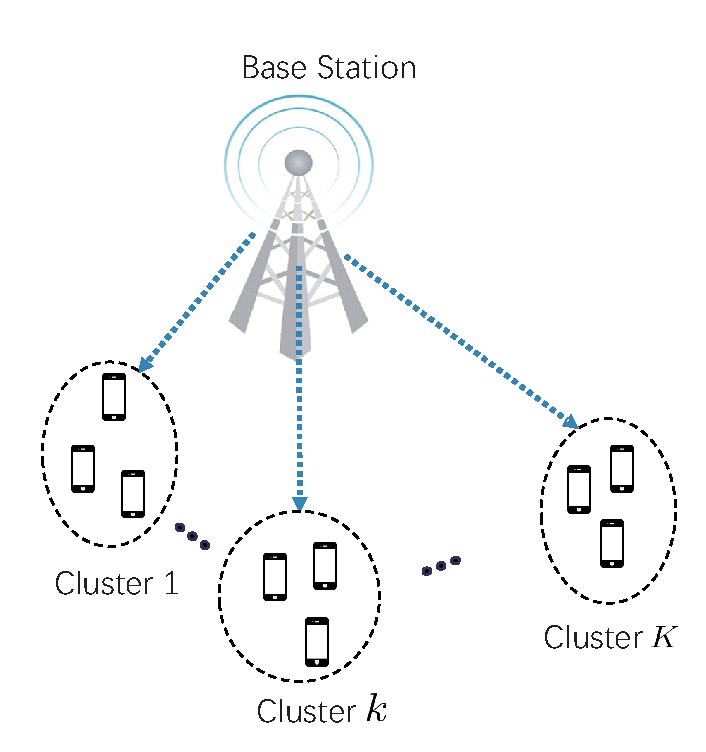
\includegraphics[scale=0.55]{PPTFigure/groupcluster.eps}
%		\caption{Group scheduling to reduce the number of RF chains and eliminate the intra-cluster interference}\label{fig:BDMA}
%	\end{center}
%\end{figure}

{\color{red}However, the number of RF chains is lower bounded by the transmitted the number of data streams. In our proposed system, the users are grouped to several clusters. We assume the symbol duration is much larger than time delay thus the received symbols of different users are same and the channel gain is constant. Compared to serve each cluster separately, the interference will increase since each user has to decode received signal from other clusters. Leveraging the scheduling of users, we can firstly use analog precoding to eliminate the inter-cluster interference between cluster and then implement digital precoding to suppress the intra-cluster interference. The simulation results show that our proposed algorithm can efficiently reduce the number of RF chains without introducing large intra-cluster interference.} 

\underline{Notation}: Vectors and matrices are denoted by boldface letters. ${\bm A}^T$ and ${\bm A}^H$ denote transpose and conjugate transpose of ${\bm A}$, respectively. $\bm{A}^\dagger$ being the pseudo inverse of $\bm{A}$ while $||\bm{A}|| $ and $|\bm{A}|$ stand for the Frobenius norm and determinant of ${\bm A}$, respectively. $\bm{A}(i,j)$ denotes the $i$ row, $j$ column element of ${\bm A}$; $|\mathcal{I}|$ is the cardinality of the enclosed set ${\cal I}$; Finally, $\mathbb{E}[\cdot] $ and $\Re\{\cdot\}$ denote the expectation and real part of a random variable.

%\begin{figure*}[htpb]
%	\centering
%	\begin{minipage}[t]{0.7\linewidth}
%		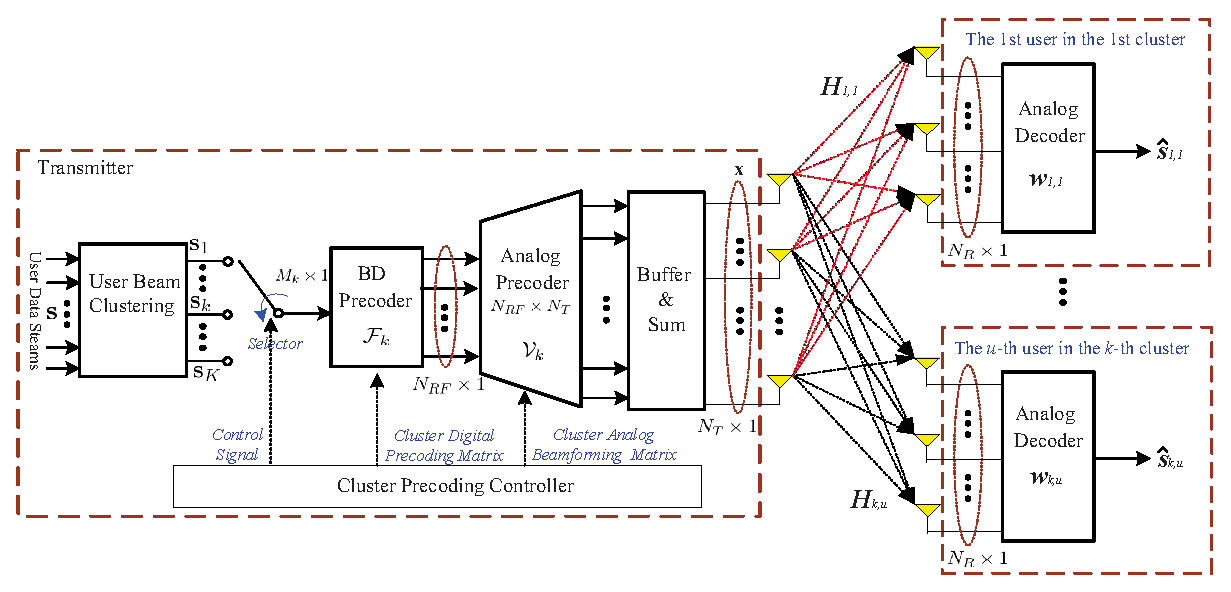
\includegraphics[width=5.6in,height=3in]{PPTFigure/BlockDiagonal.eps}
%		\caption{Block diagram of the hybrid precoding system under consideration}\label{fig:BlockDiagram}
%		\parbox{6.5cm}{\small \hspace{1.5cm} }
%	\end{minipage}
%\end{figure*}

\section{system model}
%There are $N_{tot}$ users under considered base station, and $N_U$ of them will be selected to serve. We consider a multi-user mmWave MIMO system shown in \figurename{ \ref{fig:BlockDiagram}}, in which a transmitter equipped with $N_{RF}$ RF chains and $N_T$ antennas transmits $N_U$ data streams to $N_U$ receivers with $N_R$ receive antennas. Following the same assumption commonly employed in the literature \cite{alkhateeb2015limited}, we assume only one data stream is designated to each scheduled receiver. We use ${\bm s}(n)$ to denote the $n$-th block of $N_U$ data to be transmitted with $\mathbb{E}\left[\bm{ss}^H\right]=\frac{1}{N_U}\bm{I}_{N_U}$. In the sequel, we concentrate on a single block and omit the temporal index $n$ for notational simplicity.


\subsection{problem formulation}

precoded signal:
\begin{equation}{\label{eq:transx1}}
{\bm x} = \bm{V}\bm{F}\bm{s}
\end{equation}


received signal:
\begin{eqnarray}{\label{eq:rewrite}}
{\bm y}_{u} &=&\underbrace{\bm{H}_{u} \bm{V}\bm{f}_{u}{s}_{u}}_\text{Desired Signal}+\underbrace{\bm{H}_{u} \bm{V}\sum_{\substack{i=1 \\ i\neq u}}^{N_U}\bm{f}_{i}s_{i}}_\text{Interference}+\underbrace{\bm{n}_{u}}_\text{Noise}
\end{eqnarray}

decoded signal:
\begin{equation}
\hat{s}_{u} = \bm{w}_{u}^H \bm{H}_{u} \bm{V} \bm{f}_{u} s_{u} + \bm{w}_{u}^H \bm{\tilde{n}}_{u},
\end{equation}
where,
\begin{equation}
\bm{\tilde{n}}_u=\bm{H}_{u} \bm{V}\sum_{\substack{i=1 \\ i\neq u}}^{N_U}\bm{f}_{i}s_{i} + \bm{n}_{u}.
\end{equation}

let
\begin{equation}
{\bm{g}}_{u}^H = \bm{w}^H_{u} \bm{H}_{u} \bm{V}.
\end{equation}

data rate:
\begin{equation}
R_{u} = \log\left(1+\frac{P}{N_U}|{\bm{g}}_{u}^H \bm{f}_{u}|^2\left(\frac{P}{N_U}\displaystyle\sum_{\substack{i=1 \\ i\neq u}}^{N_U}|{\bm{g}}_{u}^H\bm{f}_{i}|^2+\sigma^2\right)^{-1}\right).
\end{equation}

average rate:
\begin{equation}
R_{avg}=\frac{1}{KN_U}\sum_{k=1}^{K}\sum_{u=1}^{N_U}R_{u}.
\end{equation}


Problem:
\begin{equation}
\begin{aligned}
P1:\qquad&\max_{\bm V,\bm F} \quad R_{avg}\\
s.t. \quad& C1:\mathrm{tr}\left(\bm V\bm V^H\right)\leq 1,\\
\quad& C2:\mathrm{tr}\left(\bm F\bm F^H\right)\leq 1,\\
\quad& C3:N_{RF}\leq \bar{N}_{RF},
\end{aligned}
\end{equation}

\subsection{Channel Model}
As shown in \cite{rappaport2014millimeter}, the mmWave wireless channel can be well modeled by the Saleh-Valenzuela model. Following the same approach developed in \cite{alkhateeb2014channel}, we assume that each scatter only contributes one single propagation path. As a result, the $u$-th user's channel model can been modeled as:
\begin{equation}{\label{eq:Hu}}
\bm{H}_u = \sqrt{\frac{N_{T}N_{R}}{L_{u}}}\sum_{l=1}^{L_u}\alpha_{u,l}\cdot \bm{a}_{R}(\phi^r_{u,l},\theta^r_{u,l}) \cdot\bm{a}_{T}^{H}(\phi^t_{u,l},\theta^t_{u,l}),
\end{equation}
where $L_u$ is the number of scatters of the $u$-th user's channel. Furthermore, $\alpha_{u,l}$, $\theta^r_{u,l}/\phi^r_{u,l}$ and $\theta^t_{u,l}/\phi^t_{u,l}$ are the complex path gain, azimuth/elevation angles of arrival(AoA) and azimuth/elevation angles of departure(AoD) of the $l$-th path of the $u$-th user, respectively. Finally, ${\bm a}$ is the array response vector. For an uniform planar array (UPA) of size $P\times Q$ considered in this work, the array response vector ${\bm a}$ is given by \cite{alkhateeb2014channel}
\begin{flalign}\label{eq:UPAvec1}
\bm{a}(\phi,\theta) =&\frac{1}{\sqrt{N_T}}\left[1,  e^{jkd(\sin\phi \sin\theta +\cos\theta)},\cdots,\right.&&\nonumber\\
&\left. e^{jkd\left(p\sin\phi \sin\theta +q\cos\theta\right)},\cdots, \right. &&\nonumber\\
&\left. e^{jkd\left((P-1)\sin\phi \sin\theta +(Q-1)\cos\theta\right)}\right]^T,&&
\end{flalign}
where $k=\frac{2\pi}{\lambda}$ is the wavenumber while $d$ is the distance between two adjacent antennas.

\section{PROPOSED BLOCK HYBRID BEAMFORMING}
\subsection{When $N_U\leq\bar{N}_{RF}$,ZF precoder}
ZF precoder stuff goes here.

\subsection{When $N_U>\bar{N}_{RF}$,Block Diagonal Digital Precoder}
Divide users into $K$ clusters.

\begin{equation}
\bm{s} = \left[{\mathbf{s}}_1^T, {\mathbf{s}}_2^T,\cdots, \mathbf{s}_{K}^T\right]^T, \quad \mathbf{s}_k\in \mathcal{C}^{M_j\times 1}
\end{equation}

$K$ digital precoders for $K$ clusters:
\begin{equation}
\bm{\mathcal{F}} = \left[\bm{\mathcal{F}}_1, \bm{\mathcal{F}}_2,\cdots, \bm{\mathcal{F}}_{K}\right], \quad \bm{\mathcal{F}}_k\in \mathcal{C}^{N_T\times M_k}
\end{equation}

$K$ analog precoders for $K$ clusters:
\begin{equation}
\bm{\mathcal{V}} = \left[\bm{\mathcal{V}}_1, \bm{\mathcal{V}}_2,\cdots, \bm{\mathcal{V}}_{K}\right], \quad \bm{\mathcal{V}}_k\in \mathcal{C}^{N_T\times M_k}
\end{equation}

precoded signal of $k$-th cluster:
\begin{equation}
{\bm x}_{k} = \bm{\mathcal{V}}_k \bm{\mathcal{F}}_k \mathbf{s}_k
\end{equation}

radiated signal is equal to the sum of all precoded signals:
\begin{equation}
{\bm x}= \sum_{k=1}^K \bm{\mathcal{V}}_k \bm{\mathcal{F}}_k \mathbf{s}_k = \bm{V}\bm{F}\bm{s}
\end{equation}
where,

\begin{equation}
\bm{F} = 
\begin{bmatrix}
\bm{\mathcal{F}}_1&\cdots & \bm{0}&\bm{0}\\
\vdots & \bm{\mathcal{F}}_2 & \vdots&\vdots \\
\bm{0}&\cdots&\ddots &\bm{0}\\
\bm{0}&\cdots & \bm{0}&\bm{\mathcal{F}}_K
\end{bmatrix}
,\bm{V} = 
\begin{bmatrix}
\bm{{\mathcal{V}}}_1&\cdots & \bm{0}&\bm{0}\\
\vdots & \bm{\mathcal{V}}_2 & \vdots&\vdots \\
\bm{0}&\cdots&\ddots &\bm{0}\\
\bm{0}&\cdots & \bm{0}&\bm{\mathcal{V}}_K
\end{bmatrix}
\end{equation}

received signal of $u$-th user in $k$-th cluster:
\begin{eqnarray}{\label{eq:rewrite}}
{\bm y}_{ku} &=&\underbrace{\bm{H}_{ku} \bm{\mathcal{V}}_k\bm{f}_{ku}{s}_{ku}}_\text{Desired Signal}+\underbrace{\bm{H}_{ku} \bm{\mathcal{V}}_k\sum_{\substack{i=1 \\ i\neq u}}^{M_K}\bm{f}_{ki}s_{ki}}_\text{Intra-cluster Interference} \nonumber\\
&+& \underbrace{\bm{H}_{ku}\sum_{\substack{j=1\\j\neq k}}^{K}\bm{\mathcal{V}}_j\bm{F}_j\bm{s}_j}_\text{Inter-cluster Interference}+ \underbrace{\bm{n}_{ku}}_\text{Noise}
\end{eqnarray}

decoded signal
\begin{equation}{\label{eq:hats}}
\hat{s}_{ku} = \bm{w}_{ku}^H \bm{H}_{ku} \bm{\mathcal{V}}_k \bm{f}_{ku} s_{ku} + \bm{w}_{ku}^H \bm{\tilde{n}}_{ku},
\end{equation}

\begin{equation}\label{Eq:ntilde}
\bm{\tilde{n}}_{ku}=\bm{H}_{ku} \bm{\mathcal{V}}_k\sum_{\substack{i=1 \\ i\neq u}}^{M_K}\bm{f}_{ki}s_{ki} + \bm{H}_{ku}\sum_{\substack{j=1\\j\neq k}}^{K}\bm{\mathcal{V}}_j\bm{\mathcal{F}}_j\bm{s}_j+ \underbrace{\bm{n}_{ku}}_\text{Noise}
\end{equation}

let
\begin{equation}\label{eq:defgu}
{\bm{g}}_{ku}^H = \bm{w}^H_{ku} \bm{H}_{ku} \bm{\mathcal{V}}_{k}.
\end{equation}

\begin{equation}\label{eq:def}
{\bm{t}}_{ku,j}^H = \bm{w}^H_{ku} \bm{H}_{ku} \bm{\mathcal{V}}_{j}.
\end{equation}

data rate:
\begin{equation}
\begin{aligned}
R_{ku} &= \\
&\log\left(1+\frac{\frac{P}{N_U}|{\bm{g}}_{ku}^H \bm{f}_{ku}|^2}{
\sum_{\substack{i=1 \\ i\neq u}}^{M_k}\left|{\bm{g}}_{ku}^H\bm{f}_{ki}\right|^2+\sum_{\substack{j=1\\j\neq k}}^{K}\|\bm{t}_{ku,j}\bm{\mathcal{F}}_j\|^2+\sigma^2}\right).
\end{aligned}
\end{equation}


Problem is equivalently convert to:
\begin{equation}
\begin{aligned}
P2:\qquad&\max_{\bm V,\bm F} \quad R_{avg}\\
s.t. & \quad C1,C2,\\
&\quad C4:\bm{F}=\mathrm{diag}\{\bm{\mathcal{F}}_k\},\ \bm{\mathcal{F}}_k\in \mathcal{C}^{N_T\times M_k},\\
&\quad C5:\bm{V}=\mathrm{diag}\{\bm{\mathcal{V}}_k\},\ \bm{\mathcal{V}}_k\in \mathcal{C}^{N_T\times M_k},\\
&\quad C6:\max \{M_k\}_{k=1}^K\leq \bar{N}_{RF},
\end{aligned}
\end{equation}

we can solve the above problem by...


\section{USER CLUSTERING AND POWER ALLOCATION}
\subsection{Heuristic user clustering}

\begin{algorithm}[h] 		
	\caption{Greedy scheduling algorithm for PAPR-aware hybrid beamforming}
	\label{selection}
	\begin{algorithmic}
		\REQUIRE  \quad
		\STATE	All user index set: $\mathcal{X}$\\
		\STATE  Selected user index set : $\mathcal{I}_k=\emptyset$, $k=1,2,\cdots, K$\\
		\STATE  Number of clusters: $K$\\
		\STATE  Analog precoder solved by Eq. \eqref{eq:analogprecoder}: $\bm{V}=[\bm{v}_1,\bm{v}_2,\cdots,\bm{v}_{N_U}]$
		\ENSURE   	
		\STATE Initialization: Assign the user index $x$ corresponding to the largest channel gain $|\alpha|$ to ${\mathcal I}_1$, {\em i.e.} $\mathcal{I}_1 \leftarrow  x$ and ${\mathcal X}\setminus x$, 
		\STATE $\bm{V}_{else} = [v_1]$
		\FOR{$x$ in $\mathcal{x}$}
		\STATE $p(x) = $
		\ENDFOR
		\WHILE{$|{\cal I}|< N_U$}
		\STATE ${\bm A}=\left[\bm{a}_{T}\left(\phi^t_{i_1},\theta^t_{i_1}\right),\bm{a}_{T}\left(\phi^t_{i_2},\theta^t_{i_2}\right),\cdots,\bm{a}_{T}\left(\phi^t_{i_{|{\cal I}|}},\theta^t_{i_{|{\cal I}|}}\right)\right]$
		\STATE Compute the projection space: ${\bm P}_A = {\bm A}{\bm A}^{\dagger}$ 		 				
		\FOR{$x$ in {$\mathcal{X}$}}
		\STATE $p(x) = \|{\bm P}_A\cdot {\bm a}_T\left(\phi^t_{x},\theta^t_{x}\right)\|^2$ 				 								
		\ENDFOR
		\STATE  Find the user index $x^*$ with the minimum $p(x)$ 									
		\STATE	Update ${\cal I} \leftarrow  x^*$ and ${\cal X}\setminus x^*$	
		\ENDWHILE	
	\end{algorithmic}
\end{algorithm}

\subsection{Power Allocation for SIR}

In this section, we will discuss the power allocation of multi-user MIMO system. For high signal-to-noise(SNR) ratio scenario, the noise can be ignored. The powers for users are represented as $\bm{p}=[p_1, p_2, \cdots, p_{N_U}]$. 

The SIR of $u$-th user is set to be 
\begin{align}
\gamma_u &= \frac{p_u|\bm{g}_u^H\bm{f}^*_{ZF,u}|^2}{\sum_{i\neq u}^{N_U}p_i|\bm{g}_u^H \bm{f}^*_{ZF,i}|^2} \nonumber\\
&= \frac{p_u|\bm{g}_u^H\bm{f}^*_{ZF,u}|^2}{\sum_{i=1}^{N_U}p_i|\bm{g}_u^H \bm{f}^*_{ZF,i}|^2 - p_u|\bm{g}_u^H \bm{f}^*_{ZF,u}|^2}
\end{align}

Considering the balanced SIR theory 
\begin{equation}
\gamma_u=\gamma, u=1,2,\cdots,N_U
\end{equation}

the transmitted power can be minimized by eigenvalue problem
\begin{equation}
\bm{Gp} = \frac{\gamma+1}{\gamma} \bm{p}
\end{equation}
where 
\begin{equation}
\bm{G}=
\begin{bmatrix}
1&T_2/T_1&\cdots&T_{N_U}/T_1\\
T_1/T_2&1&\cdots&T_{N_U}/T_2\\
\cdots&\cdots&\cdots&\cdots\\
T_1/T_{N_U}&T_2/T_{N_U}&\cdots&1
\end{bmatrix}
\end{equation}
and
\begin{equation}
T_u = |\bm{g}_u^H \bm{f}^*_{ZF,u}|^2
\end{equation}
This problem can be easily solved by 
\begin{equation}
\gamma = \frac{1}{\lambda_{max}(\bm{G})-1}
\end{equation}

As the elements of $\bm{G}$ are positive, from the \textit{Perron Frobenius Theorem}, we know there must exist at least one positive eigenvector and thus the power is solved.

\bibliography{BDMAref}
\bibliographystyle{IEEEtran}


% references section

\end{document}


